% I seguenti commenti speciali impostano:
% 1. 
% 2. PDFLaTeX come motore di composizione;
% 3. tesi.tex come documento principale;
% 4. il controllo ortografico italiano per l'editor.

% !TEX encoding = UTF-8
% !TEX TS-program = pdflatex
% !TEX root = tesi.tex
% !TeX spellcheck = en_GB

\documentclass[10pt,                    % corpo del font principale
               a4paper,                 % carta A4
               twoside,                 % impagina per fronte-retro
               openright,               % inizio capitoli a destra
               english,                 
               italian,                 
               ]{book}    

%**************************************************************
% Importazione package
%************************************************************** 

%\usepackage{amsmath,amssymb,amsthm}    % matematica

\usepackage[T1]{fontenc}                % codifica dei font:
                                        % NOTA BENE! richiede una distribuzione *completa* di LaTeX

\usepackage[utf8]{inputenc}             % codifica di input; anche [latin1] va bene
                                        % NOTA BENE! va accordata con le preferenze dell'editor

\usepackage[english, italian]{babel}    % per scrivere in italiano e in inglese;
                                        % l'ultima lingua (l'italiano) risulta predefinita

\usepackage{bookmark}                   % segnalibri

\usepackage{caption}                    % didascalie

\usepackage{chngpage,calc}              % centra il frontespizio

\usepackage{csquotes}                   % gestisce automaticamente i caratteri (")

\usepackage{emptypage}                  % pagine vuote senza testatina e piede di pagina

\usepackage{epigraph}			% per epigrafi

\usepackage{eurosym}                    % simbolo dell'euro

%\usepackage{indentfirst}               % rientra il primo paragrafo di ogni sezione

\usepackage{graphicx}                   % immagini

\usepackage{hyperref}                   % collegamenti ipertestuali

\usepackage[binding=5mm]{layaureo}      % margini ottimizzati per l'A4; rilegatura di 5 mm

\usepackage{listings}                   % codici

\usepackage{microtype}                  % microtipografia

\usepackage{mparhack,fixltx2e,relsize}  % finezze tipografiche

\usepackage{nameref}                    % visualizza nome dei riferimenti                                      

\usepackage[font=small]{quoting}        % citazioni

\usepackage{subfig}                     % sottofigure, sottotabelle

\usepackage[italian]{varioref}          % riferimenti completi della pagina

\usepackage[dvipsnames]{xcolor}         % colori

\usepackage{booktabs}                   % tabelle                                       
\usepackage{tabularx}                   % tabelle di larghezza prefissata                                    
\usepackage{longtable}                  % tabelle su più pagine                                        
\usepackage{ltxtable}                   % tabelle su più pagine e adattabili in larghezza
\usepackage{lmodern}
\usepackage[toc, acronym]{glossaries}   % glossario
                                        % per includerlo nel documento bisogna:
                                        % 1. compilare una prima volta tesi.tex;
                                        % 2. eseguire: makeindex -s tesi.ist -t tesi.glg -o tesi.gls tesi.glo
                                        % 3. eseguire: makeindex -s tesi.ist -t tesi.alg -o tesi.acr tesi.acn
                                        % 4. compilare due volte tesi.tex.

\usepackage[backend=biber,style=verbose-ibid,hyperref,backref]{biblatex}
                                        % eccellente pacchetto per la bibliografia; 
                                        % produce uno stile di citazione autore-anno; 
                                        % lo stile "numeric-comp" produce riferimenti numerici
                                        % per includerlo nel documento bisogna:
                                        % 1. compilare una prima volta tesi.tex;
                                        % 2. eseguire: biber tesi
                                        % 3. compilare ancora tesi.tex.

%**************************************************************
% file contenente le impostazioni della tesi
%**************************************************************

%**************************************************************
% Frontespizio
%**************************************************************

% Autore
\newcommand{\myName}{Stefano Panozzo}                                    
\newcommand{\myTitle}{Introduzione al big data computing ed una sua applicazione}

% Tipo di tesi                   
\newcommand{\myDegree}{Tesi di laurea triennale}

% Università             
\newcommand{\myUni}{Università degli Studi di Padova}

% Facoltà       
\newcommand{\myFaculty}{Corso di Laurea in Informatica}

% Dipartimento
\newcommand{\myDepartment}{Dipartimento di Matematica "Tullio Levi-Civita"}

% Titolo del relatore
\newcommand{\profTitle}{Prof.}

% Relatore
\newcommand{\myProf}{Tullio Vardanega}

% Luogo
\newcommand{\myLocation}{Padova}

% Anno accademico
\newcommand{\myAA}{2017-2018}

% Data discussione
\newcommand{\myTime}{Dicembre 2018}


%**************************************************************
% Impostazioni di impaginazione
% see: http://wwwcdf.pd.infn.it/AppuntiLinux/a2547.htm
%**************************************************************

\setlength{\parindent}{14pt}   % larghezza rientro della prima riga
\setlength{\parskip}{0pt}   % distanza tra i paragrafi


%**************************************************************
% Impostazioni di biblatex
%**************************************************************
\bibliography{bibliografia} % database di biblatex 

\defbibheading{bibliography} {
    \cleardoublepage
    \phantomsection 
    \addcontentsline{toc}{chapter}{\bibname}
    \chapter*{\bibname\markboth{\bibname}{\bibname}}
}

\setlength\bibitemsep{1.5\itemsep} % spazio tra entry

\DeclareBibliographyCategory{opere}
\DeclareBibliographyCategory{web}

\addtocategory{opere}{womak:lean-thinking}
\addtocategory{web}{site:agile-manifesto}

\defbibheading{opere}{\section*{Riferimenti bibliografici}}
\defbibheading{web}{\section*{Siti Web consultati}}


%**************************************************************
% Impostazioni di caption
%**************************************************************
\captionsetup{
    tableposition=top,
    figureposition=bottom,
    font=small,
    format=hang,
    labelfont=bf
}

%**************************************************************
% Impostazioni di glossaries
%**************************************************************

%**************************************************************
% Acronimi
%**************************************************************
\renewcommand{\acronymname}{Acronimi e abbreviazioni}
%**************************************************************
% Glossario
%**************************************************************
%\renewcommand{\glossaryname}{Glossario}

\newglossaryentry{apig}
{
    name=API,
    text=Application Program Interface,
    sort=api,
    description={insieme di procedure disponibili al programmatore, di solito raggruppate a formare un set di strumenti specifici per l'espletamento di un determinato compito all'interno di un certo programma. La finalità è ottenere un'astrazione, di solito tra l'hardware e il programmatore o tra software a basso e quello ad alto livello semplificando così il lavoro di programmazione}
}

\newglossaryentry{cluster}
{
    name=Cluster,
    text=cluster,
    sort=cluster,
    description={(indicato anche come computer cluster) insieme di macchine connesse tra loro che lavorano in parallelo.
    L'utilizzo di questi sistemi permette di distribuire un'elaborazione molto complessa tra le varie macchine, aumentando la potenza di calcolo del sistema e/o garantendo una maggiore disponibilità di servizio, a prezzo di un maggior costo e complessità di gestione dell'infrastruttura: per essere risolto, il problema che richiede molte elaborazioni, viene infatti scomposto in sottoproblemi separati i quali vengono risolti ciascuno in parallelo su tutti i nodi che compongono il cluster}
}

\newglossaryentry{web app}
{
	name=Web App,
	text=web app,
	sort=web app,
	description={sistema di tipo client-server in cui l'interfaccia utente e la logica client-side viene eseguita in un browser web}
}

\newglossaryentry{SDLC}
{
	name=Software Development Lifecycle,
	text=Software Development Lifecycle,
	sort=SDLC,
	description={processo di divisione del lavoro di sviluppo software in fasi distinte per migliorare la progettazione, la gestione del prodotto e la gestione del progetto}
}

\newglossaryentry{MVP}
{
	name=Minimum Viable Product,
	text=Minimum Viable Product,
	sort=MVP,
	description={prototipo più semplificato possibile che è possibile presentare ad una cerchia di possibili clienti (early adopter). È il mezzo con cui testare e validare le idee e il prodotto stesso, senza sprecare tempo e soldi a sviluppare il prodotto completo, per poi constatare che quel prodotto non interessa alla clientela}
}

\newglossaryentry{Bash}{bash}
{
	name=Bash,
	text=Bash,
	sort=Bash,
	description={shell testuale del progetto GNU usata nei sistemi operativi Unix e Unix-like, specialmente in GNU/Linux. Si tratta di un interprete di comandi che permette all'utente di comunicare col sistema operativo attraverso una serie di funzioni predefinite, o di eseguire programmi e script.\\		
	Bash è in grado di eseguire i comandi che le vengono passati, utilizzando la redirezione dell'input e dell'output per eseguire più programmi in cascata in una pipeline software, passando l'output del comando precedente come input del comando successivo.
	Oltre a questo, essa mette a disposizione un semplice linguaggio di scripting nativo che permette di svolgere compiti più complessi, non solo raccogliendo in uno script una serie di comandi, ma anche utilizzando variabili, funzioni e strutture di controllo di flusso}
}

\newglossaryentry{Git}
{
	name=Git,
	text=Git,
	sort=Git,
	description={Git è un software di controllo versione distribuito utilizzabile da interfaccia a riga di comando, creato da Linus Torvalds nel 2005 con lo scopo di essere un semplice strumento per facilitare lo sviluppo del kernel Linux, e diventato poi uno degli strumenti di controllo versione più diffusi al mondo}
}

\newglossaryentry{GitLab}
{
	name=GitLab,
	text=GitLab,
	sort=GitLab,
	description={GitLab è un manager di \textit{repository} Git basato su interfaccia web, che include anche funzioni quali una wiki per ogni progetto e un sistema di tracciamento issue. Esso è stato sviluppato da GitLab Inc. ed è distribuito gratuitamente con licenza \textit{open source}}
}

\newglossaryentry{IDE}
{
	name=IDE,
	text=IDE,
	sort=IDE,
	description={(in lingua inglese \textit{Integrated Development Environment} ovvero IDE, anche \textit{integrated design environment} o \textit{integrated debugging environment}, rispettivamente ambiente integrato di progettazione e ambiente integrato di \textit{debugging}) è un software che, in fase di programmazione, aiuta i programmatori nello sviluppo del codice sorgente di un programma. Spesso l’IDE aiuta lo sviluppatore segnalando errori di sintassi del codice direttamente in fase di scrittura, oltre a tutta una serie di strumenti e funzionalità di supporto alla fase di sviluppo e \textit{debugging}}
}

\newglossaryentry{Single Customer View}
{
	name=Single Customer View,
	text=Single Customer View,
	sort=Single Customer View,
	description={rappresentazione olistica del cliente che integra tutti i dati e gli eventi del cliente, e consente di arrivare ad un’interpretazione completa e contestuale dei suoi comportamenti indipendentemente dai canali utilizzati}
}

\newglossaryentry{Web Service}
{
	name=Web Service,
	text=Web Service,
	sort=Web Service,
	description={sistema software in grado di mettersi al servizio di un applicazione comunicando su di una medesima rete tramite il protocollo HTTP. Un Web service consente quindi alle applicazioni che vi si collegano di usufruire delle funzioni che mette a disposizione}
}

\newglossaryentry{HDFS}
{
	name=HDFS,
	text=HDFS,
	sort=HDFS,
	description={Hadoop Distributed File System è un file system distribuito, portabile e scalabile scritto in Java per il framework Hadoop. Un cluster in Hadoop tipicamente possiede un singolo NameNode (su cui risiedono i metadati dei file) e un insieme di DataNode (su cui risiedono, in blocchi di dimensione fissa, i file dell'HDFS)}
}

\newglossaryentry{Diagramma di Gantt}
{
	name=Diagramma di Gantt,
	text=Diagramma di Gantt,
	sort=Diagramma di Gantt,
	description={Il diagramma di Gantt è uno strumento di supporto alla gestione dei progetti, così chiamato in ricordo dell'ingegnere statunitense Henry Laurence Gantt (1861-1919), che si occupava di scienze sociali e che lo ideò nel 1917. Tale diagramma è usato principalmente nelle attività di \textit{project management}, ed è costruito partendo da un asse orizzontale - a rappresentazione dell'arco temporale totale del progetto, suddiviso in fasi incrementali (ad esempio: giorni, settimane, mesi) - e da un asse verticale - a rappresentazione delle mansioni o attività che costituiscono il progetto}
} % database di termini
\makeglossaries


%**************************************************************
% Impostazioni di graphicx
%**************************************************************
\graphicspath{{immagini/}} % cartella dove sono riposte le immagini


%**************************************************************
% Impostazioni di hyperref
%**************************************************************
\hypersetup{
    %hyperfootnotes=false,
    %pdfpagelabels,
    %draft,	% = elimina tutti i link (utile per stampe in bianco e nero)
    colorlinks=true,
    linktocpage=true,
    pdfstartpage=1,
    pdfstartview=FitV,
    % decommenta la riga seguente per avere link in nero (per esempio per la stampa in bianco e nero)
    %colorlinks=false, linktocpage=false, pdfborder={0 0 0}, pdfstartpage=1, pdfstartview=FitV,
    breaklinks=true,
    pdfpagemode=UseNone,
    pageanchor=true,
    pdfpagemode=UseOutlines,
    plainpages=false,
    bookmarksnumbered,
    bookmarksopen=true,
    bookmarksopenlevel=1,
    hypertexnames=true,
    pdfhighlight=/O,
    %nesting=true,
    %frenchlinks,
    urlcolor=webbrown,
    linkcolor=RoyalBlue,
    citecolor=webgreen,
    %pagecolor=RoyalBlue,
    %urlcolor=Black, linkcolor=Black, citecolor=Black, %pagecolor=Black,
    pdftitle={\myTitle},
    pdfauthor={\textcopyright\ \myName, \myUni, \myFaculty},
    pdfsubject={},
    pdfkeywords={},
    pdfcreator={pdfLaTeX},
    pdfproducer={LaTeX}
}

%**************************************************************
% Impostazioni di itemize
%**************************************************************
\renewcommand{\labelitemi}{$\ast$}

%\renewcommand{\labelitemi}{$\bullet$}
%\renewcommand{\labelitemii}{$\cdot$}
%\renewcommand{\labelitemiii}{$\diamond$}
%\renewcommand{\labelitemiv}{$\ast$}


%**************************************************************
% Impostazioni di listings
%**************************************************************
\lstset{
    language=[LaTeX]Tex,%C++,
    keywordstyle=\color{RoyalBlue}, %\bfseries,
    basicstyle=\small\ttfamily,
    %identifierstyle=\color{NavyBlue},
    commentstyle=\color{Green}\ttfamily,
    stringstyle=\rmfamily,
    numbers=none, %left,%
    numberstyle=\scriptsize, %\tiny
    stepnumber=5,
    numbersep=8pt,
    showstringspaces=false,
    breaklines=true,
    frameround=ftff,
    frame=single
} 


%**************************************************************
% Impostazioni di xcolor
%**************************************************************
\definecolor{webgreen}{rgb}{0,.5,0}
\definecolor{webbrown}{rgb}{.6,0,0}


%**************************************************************
% Altro
%**************************************************************

\newcommand{\omissis}{[\dots\negthinspace]} % produce [...]

% eccezioni all'algoritmo di sillabazione
\hyphenation
{
    ma-cro-istru-zio-ne
    gi-ral-din
}

\newcommand{\sectionname}{sezione}
\addto\captionsitalian{\renewcommand{\figurename}{Figura}
                       \renewcommand{\tablename}{Tabella}}

\newcommand{\glsfirstoccur}{\ap{{[g]}}}

\newcommand{\intro}[1]{\emph{\textsf{#1}}}

%**************************************************************
% Environment per ``rischi''
%**************************************************************
\newcounter{riskcounter}                % define a counter
\setcounter{riskcounter}{0}             % set the counter to some initial value

%%%% Parameters
% #1: Title
\newenvironment{risk}[1]{
    \refstepcounter{riskcounter}        % increment counter
    \par \noindent                      % start new paragraph
    \textbf{\arabic{riskcounter}. #1}   % display the title before the 
                                        % content of the environment is displayed 
}{
    \par\medskip
}

\newcommand{\riskname}{Rischio}

\newcommand{\riskdescription}[1]{\textbf{\\Descrizione:} #1.}

\newcommand{\risksolution}[1]{\textbf{\\Soluzione:} #1.}

%**************************************************************
% Environment per ``use case''
%**************************************************************
\newcounter{usecasecounter}             % define a counter
\setcounter{usecasecounter}{0}          % set the counter to some initial value

%%%% Parameters
% #1: ID
% #2: Nome
\newenvironment{usecase}[2]{
    \renewcommand{\theusecasecounter}{\usecasename #1}  % this is where the display of 
                                                        % the counter is overwritten/modified
    \refstepcounter{usecasecounter}             % increment counter
    \vspace{10pt}
    \par \noindent                              % start new paragraph
    {\large \textbf{\usecasename #1: #2}}       % display the title before the 
                                                % content of the environment is displayed 
    \medskip
}{
    \medskip
}

\newcommand{\usecasename}{UC}

\newcommand{\usecaseactors}[1]{\textbf{\\Attori Principali:} #1. \vspace{4pt}}
\newcommand{\usecasepre}[1]{\textbf{\\Precondizioni:} #1. \vspace{4pt}}
\newcommand{\usecasedesc}[1]{\textbf{\\Descrizione:} #1. \vspace{4pt}}
\newcommand{\usecasepost}[1]{\textbf{\\Postcondizioni:} #1. \vspace{4pt}}
\newcommand{\usecasealt}[1]{\textbf{\\Scenario Alternativo:} #1. \vspace{4pt}}

%**************************************************************
% Environment per ``namespace description''
%**************************************************************

\newenvironment{namespacedesc}{
    \vspace{10pt}
    \par \noindent                              % start new paragraph
    \begin{description} 
}{
    \end{description}
    \medskip
}

\newcommand{\classdesc}[2]{\item[\textbf{#1:}] #2}                     % file con le impostazioni personali

\begin{document}
%**************************************************************
% Materiale iniziale
%**************************************************************
\frontmatter
% !TEX encoding = UTF-8
% !TEX TS-program = pdflatex
% !TEX root = ../tesi.tex

%**************************************************************
% Frontespizio 
%**************************************************************
\begin{titlepage}

\begin{center}

\begin{LARGE}
\textbf{\myUni}\\
\end{LARGE}

\vspace{10pt}

\begin{Large}
\textsc{\myDepartment}\\
\end{Large}

\vspace{10pt}

\begin{large}
\textsc{\myFaculty}\\
\end{large}

\vspace{30pt}
\begin{figure}[htbp]
\begin{center}

\includegraphics[height=6cm]{logo-unipd}
\end{center}
\end{figure}
\vspace{30pt} 

\begin{LARGE}
\begin{center}
\textbf{\myTitle}\\
\end{center}
\end{LARGE}

\vspace{10pt} 

\begin{large}
\textsl{\myDegree}\\
\end{large}

\vspace{40pt} 

\begin{large}
\begin{flushleft}
\textit{Relatore}\\ 
\vspace{5pt} 
\profTitle \myProf
\end{flushleft}

\vspace{0pt} 

\begin{flushright}
\textit{Laureando}\\ 
\vspace{5pt} 
\myName
\end{flushright}
\end{large}

\vspace{40pt}

\line(1, 0){338} \\
\begin{normalsize}
\textsc{Anno Accademico \myAA}
\end{normalsize}

\end{center}
\end{titlepage} 
% !TEX encoding = UTF-8
% !TEX TS-program = pdflatex
% !TEX root = ../tesi.tex

%**************************************************************
% Colophon
%**************************************************************
\clearpage
\phantomsection
\thispagestyle{empty}

\hfill

\vfill

\noindent\myName: \textit{\myTitle,}
\myDegree,
\textcopyright\ \myTime.
%% !TEX encoding = UTF-8
% !TEX TS-program = pdflatex
% !TEX root = ../tesi.tex

%**************************************************************
% Dedica
%**************************************************************
\cleardoublepage
\phantomsection
\thispagestyle{empty}
\pdfbookmark{Dedica}{Dedica}

\vspace*{3cm}

\begin{center}
Perché sognare è importante, ma impegnarsi concretamente lo è ancora di più.  \\ \medskip
--- Pan di Stelle - Mulino Bianco  
\end{center}

\medskip

% !TEX encoding = UTF-8
% !TEX TS-program = pdflatex
% !TEX root = ../tesi.tex

%**************************************************************
% Sommario
%**************************************************************
\cleardoublepage
\phantomsection
\pdfbookmark{Sommario}{Sommario}
\begingroup
\let\clearpage\relax
\let\cleardoublepage\relax
\let\cleardoublepage\relax

\chapter*{Sommario}

Il presente documento descrive il lavoro svolto durante il periodo di stage del laureando Stefano Panozzo presso l'azienda I.T. Euro Consulting S.r.l. di Padova. Lo stage è stato svolto alla conclusione del percorso di studi della Laurea Triennale ed è durato in totale 320 ore.
Gli obiettivi da raggiungere erano molteplici.\\
La prima richiesta dell'azienda era analizzare la struttura del \gls{cluster} in cui risiedevano i dati utilizzati in seguito. 
Successivamente era richiesta l'analisi e la trasformazione del dataset di interesse per estrarre ed ottenere nuove informazioni utili per creare un modello che prevedesse il target desiderato. 
Infine, era richiesta la progettazione e lo sviluppo di una \gls{web app} per la rappresentazione dei risultati ottenuti in precedenza.
I primi due capitoli del presente documento hanno lo scopo di presentare il contesto aziendale in cui è stato sostenuto lo stage e di spiegare come il progetto di stage si renda utile all’interno della strategia aziendale. Il terzo capitolo documenta lo svolgimento dello stage descrivendo le attività che sono state portate a termine, i punti salienti del progetto stesso e le principali scelte progettuali. Il quarto ed ultimo capitolo presenta infine una valutazione dello svolgimento dello stage rispetto agli obiettivi aziendali e alle conoscenze acquisite dallo studente.

%\vfill
%
%\selectlanguage{english}
%\pdfbookmark{Abstract}{Abstract}
%\chapter*{Abstract}
%
%\selectlanguage{italian}

\endgroup			

\vfill


%% !TEX encoding = UTF-8
% !TEX TS-program = pdflatex
% !TEX root = ../tesi.tex

%**************************************************************
% Ringraziamenti
%**************************************************************
\cleardoublepage
\phantomsection
\pdfbookmark{Ringraziamenti}{ringraziamenti}

\begingroup
\let\clearpage\relax
\let\cleardoublepage\relax
\let\cleardoublepage\relax

\chapter*{Ringraziamenti}

\noindent \textit{Innanzitutto, vorrei esprimere la mia gratitudine al Prof. Tullio Vardanega, relatore della mia tesi, per l'aiuto e il sostegno fornitomi durante la stesura del lavoro.}\\

\noindent \textit{Desidero ringraziare con affetto i miei genitori per il sostegno, il grande aiuto e per essermi stati vicini in ogni momento durante gli anni di studio.}\\

\noindent \textit{Ho desiderio di ringraziare poi i miei amici per tutti i bellissimi anni passati insieme e le mille avventure vissute, che mi hanno fatto crescere e diventare la persona che sono ora. \\
E ringrazio la mia ragazza per avermi tradotto le mail del mio relatore (sapete, anche lei ha fatto il classico e deve tirarsela) e avermi aiutato con l'ortografia. Sì, sono una capra.} \\
\bigskip

\noindent\textit{\myLocation, \myTime}
\hfill \myName

\vspace{250pt}
\begin{flushright}{
		\slshape    
		``Perché sognare è importante, ma impegnarsi concretamente lo è ancora di più.''  \medskip} \\ 
	\medskip
	--- Pan di Stelle
\end{flushright}
\endgroup


% !TEX encoding = UTF-8
% !TEX TS-program = pdflatex
% !TEX root = ../tesi.tex

%**************************************************************
% Indici
%**************************************************************
\cleardoublepage
\pdfbookmark{\contentsname}{tableofcontents}
\setcounter{tocdepth}{2}
\tableofcontents
%\markboth{\contentsname}{\contentsname} 
\clearpage

\begingroup 
    \let\clearpage\relax
    \let\cleardoublepage\relax
    \let\cleardoublepage\relax
    %*******************************************************
    % Elenco delle figure
    %*******************************************************    
    \phantomsection
    \pdfbookmark{\listfigurename}{lof}
    \listoffigures

    \vspace*{8ex}

    %*******************************************************
    % Elenco delle tabelle
    %*******************************************************
    \phantomsection
    \pdfbookmark{\listtablename}{lot}
    \listoftables
        
    \vspace*{8ex}
\endgroup

\cleardoublepage

\cleardoublepage

%**************************************************************
% Materiale principale
%**************************************************************
\mainmatter
% !TEX encoding = UTF-8
% !TEX TS-program = pdflatex
% !TEX root = ../tesi.tex

%**************************************************************
\chapter{Il contesto aziendale}
\label{cap:introduzione}
%**************************************************************

%**************************************************************
\section{Il profilo aziendale}

IT Euro Consulting \footcite{https://www.itecons.it} è un'azienda di medie dimensioni con sede legale a Padova, nata nel 2007 e facente parte del gruppo SCAI, presente su tutto il territorio italiano. 
Dalla sua nascita si è sempre occupata prevalentemente di consulenza, \textit{System Integration} ed \textit{Application Management}, in ambito ICT, operando in tutti i principali settori di mercato: bancario ed assicurativo, industria, pubblica amministrazione e servizi.
Nel corso degli anni l'azienda ha consolidato le proprie conoscenze, offrendo svariati servizi, soprattutto nei seguenti ambiti:
\begin{itemize}
	\item \textbf{Big Data}: supporto alle aziende nel loro processo di crescita e cambiamento, tramite moderne soluzioni di \textit{Business Intelligence} e la possibilità di prevedere scenari ed eventi futuri e prendere le più opportune decisioni operative o di business grazie all'analisi della gran mole di dati che ogni giorno vengono creati. Vengono quindi offerti servizi di \textit{big data engineer}, \textit{big data scientist}, \textit{big data architect} e \textit{big data administrator};
	\item \textbf{Internet of Things}: soluzioni \textit{end-to-end}, basate su tecnologie leader di mercato che consentono di indirizzare in modo efficace la realizzazione di sistemi IoT accelerando la realizzazione di componenti web e mobile per la raccolta, la visualizzazione e l’analisi dei dati;
	\item \textbf{Reference Architecture}: intesa come \textit{best practice} e struttura di base per un insieme di domini applicativi all’interno di un’organizzazione, la quale agevola il continuo allineamento dei processi e delle strategie con le giuste soluzioni tecnologiche. Vengono quindi offerti servizi di \textit{assessment}, design e consulenza;
	\item \textbf{DevOps}: automazione delle attività manuali nelle diverse fasi del \gls{SDLC}. Il modello DevOps non si concentra esclusivamente sull’ introduzione di nuovi tool, ma è inteso come una combinazione di cultura e processi unita agli strumenti di automazione. Vengono quindi offerti servizi di \textit{assessment} e consulenza; 
	
	\begin{figure}[!h] 
		\centering 
		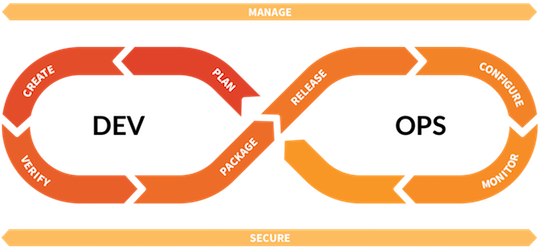
\includegraphics[width=0.6\columnwidth]{devops_lifecycle} 
		\caption{DevOps lifecycle (Fonte: \href{https://goo.gl/rh31h6}{https://goo.gl/rh31h6})}
	\end{figure}
	\newpage
	\item \textbf{System Integration}: servizi di consulenza o interventi progettuali per aiutare le aziende a gestire al meglio le proprie strutture tecnologiche complesse e soluzioni applicative per semplificare la coesione fra i vari sottosistemi che compongono la struttura;
	\item \textbf{Application Management}: servizi di manutenzione correttiva, adattativa ed evolutiva di soluzioni applicative durante il loro intero ciclo di vita;
	\item \textbf{Customer Relationship Management}: con l'obiettivo di ottenere una visione completa per perseguire uno scenario di \gls{Single Customer View}, abilitante al dialogo \textit{one-to-one} tra l'organizzazione ed il proprio cliente indipendentemente dalle canalità attraverso le quali avviene l'interazione;
	\item \textbf{System \& Data Administration}: servizio consultivo svolto avvalendosi di un insieme di strategie, processi e regole che consentono di gestire i sistemi e trattare i dati fondamentali per lo sviluppo aziendale. Vengono quindi offerti servizi di \textit{database administration}, \textit{database security}, \textit{data governance}, \textit{data analysis} e \textit{scheduling management}.
\end{itemize}

I clienti principali di IT Euro Consulting sono aziende nazionali ed internazionali che lavorano nei seguenti settori:
\begin{itemize}
	\item \textit{\textbf{Banking}};
	\item \textit{\textbf{Insurance}};
	\item \textit{\textbf{Telecommunications}};
	\item \textit{\textbf{Media \& Technology}};
	\item \textit{\textbf{Public Administration}};
	\item \textit{\textbf{Utilities \& Energy}};
	\item \textit{\textbf{Manufacturing}}.
\end{itemize}
L'azienda è quindi presente in ambienti eterogenei e di grande importanza, sia per la società che per l'impatto sociale in cui questi settori operano, i quali sono agente di innovazione per lo sviluppo futuro aziendale.

%**************************************************************
\section{Tecnologie utilizzate}

Per la realizzazione dei propri prodotti, l'azienda utilizza tecnologie che si possono raggruppare in due macro-sezioni, ovvero riguardanti lo sviluppo software e le attività inerenti ai \textit{big data}.
Per quanto concerne la prima, si può suddividere ulteriormente in due aree: \textit{back-end} e \textit{front-end}.

\subsection{Sviluppo software}
\textbf{Back-end}: per lo sviluppo del \textit{back-end} dei propri prodotti, l'azienda ha scelto il linguaggio Java, in particolare utilizzando le specifiche fornite dalla versione \textit{Enterprise Edition}\footcite{https://www.oracle.com/technetwork/java/javaee}. Questo linguaggio offre infatti un buon livello di controllo degli accessi e sicurezza per applicativi delicati come quelli in ambito bancario e assicurativo;\\\\
\textbf{Front-end}: per lo sviluppo del \textit{front-end}, l'azienda utilizza prevalentemente il \textit{framework} TypeScript Angular\footcite{https://angular.io/}, in quanto offre grande elasticità d'impiego e buone prestazioni. \\

\subsection{Big Data}
\textbf{Hadoop}\footcite{https://hadoop.apache.org/}: l'azienda utilizza questo \textit{framework} per la gestione del \gls{cluster}; Hadoop supporta applicazioni distribuite con elevato accesso ai dati, strutturati tramite il \textit{filesystem} chiamato \gls{HDFS}. Permette alle applicazioni di lavorare con migliaia di nodi e petabyte di dati;\\
\textbf{Hive}\footcite{https://hive.apache.org/}: l'azienda utilizza questo tool per effettuare le \textit{query} e l'analisi preliminare dei dati in \textit{dataset} di grandi dimensioni;\\
\textbf{Impala}\footcite{https://impala.apache.org/}: simile ad Hive, ma fornisce prestazioni leggermente migliori a discapito di una minor affidabilità e peggior gestione degli errori; \\
\textbf{Spark}\footcite{https://spark.apache.org/}: \textit{framework} per il calcolo distribuito di dati strutturati in un \gls{cluster}. Supporta applicazioni scritte in molteplici linguaggi, quelli utilizzati in azienda sono principalmente Scala e Python;\\
\textbf{R}\footcite{https://www.r-project.org/}: linguaggio di programmazione e ambiente di sviluppo specifico per l'analisi statistica dei dati, utilizzato per la stima di modelli predittivi partendo dai dati ricavati utilizzando i precedenti strumenti;\\
\textbf{Python}\footcite{https://www.python.org/}: grazie alla sua elasticità ed ai suoi svariati utilizzi, l'azienda utilizza il linguaggio Python per scopi analoghi al precedente strumento. Essendo la sintassi di questo linguaggio molto semplice, è ultimamente preferito a R.\\
\begin{figure}[!h] 
	\centering 
	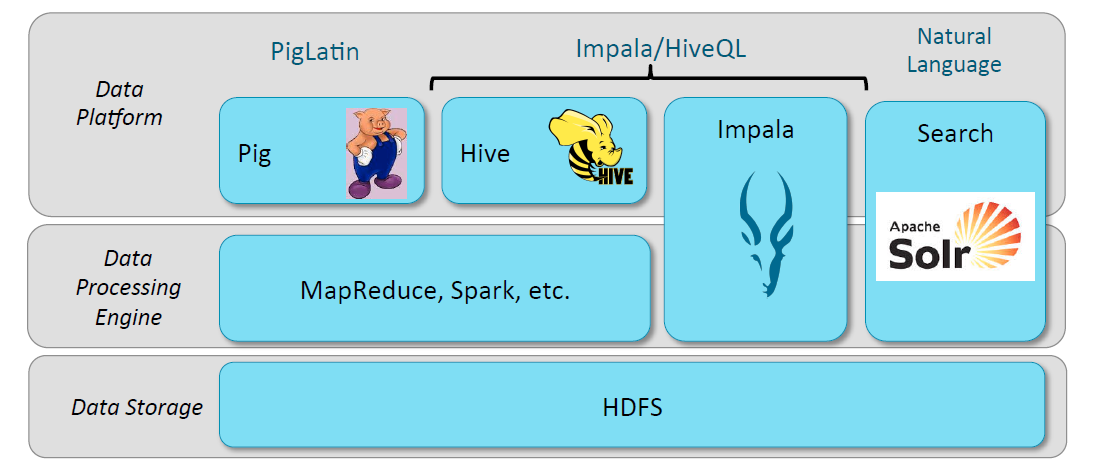
\includegraphics[width=0.9\columnwidth]{applicazioni_hadoop} 
	\caption{Esempio di tool Hadoop (Fonte: Cloudera - Data Analyst Training)}
\end{figure}

\newpage
%**************************************************************
\section{Processi aziendali}

L'azienda svolge il suo operato in base alla tipologia di lavoro da effettuare. Oltre ad eseguire progetti per un possibile cliente, sono attivi progetti per lo sviluppo di nuovo prodotto, dopo aver effettuato le ricerche di mercato d'interesse, da consegnare poi al reparto marketing per trovare compratori interessati; spesso, inoltre, l'azienda attiva dei progetti in seguito all'interesse relativo ad alcune gare d'appalto, principalmente per il settore privato ma in passato anche per quello pubblico.

\subsection{Metodologia di sviluppo}

\subsubsection{Sviluppo su commissione} \label{commissione}
Per quanto riguarda i progetti relativi allo sviluppo di un nuovo prodotto a seguito di una richiesta da parte del cliente, sotto la supervisione di un \textit{project manager} per coordinare i lavori ed interfacciarsi con il \textit{management} aziendale, il personale svolge le seguenti attività:
\begin{enumerate}
	\item \textbf{Analisi}: svolta in contemporanea dagli analisti e dal reparto marketing per il contatto con il cliente. Solitamente il personale cerca di partire da prodotti già sviluppati in azienda per poi personalizzarli in base alle richieste del cliente, così da poter offrire soluzioni già di base consolidate e testate in molteplici situazioni. Questo è preferibile soprattutto se le applicazioni sottostanti hanno bisogno di una maggior sicurezza, com'è il caso in ambito finanziario, anche per poter effettuare una manutenzione rapida in caso di malfunzionamenti.\\
	Il reparto marketing mantiene la maggior parte delle relazioni con il cliente finale all'inizio del rapporto, anche se un colloquio diretto di tecnici specializzati è ovviamente necessario dopo le prime interazioni per poter adottare soluzioni più specifiche e tecnicamente più complesse in base alle necessità del cliente;
	\item \textbf{Implementazione}: dopo aver identificato i requisiti assieme al cliente, il team incaricato si occupa dell'implementazione del prodotto concordato. Solitamente, per ogni progetto, sono assegnate un certo numero di persone e risorse per occuparsi del \textit{back-end} e del \textit{front-end} in base alla complessità ed alle tempistiche del progetto; in base alla tipologia ed alla necessità, questi saranno affiancati anche dal team che si occupa di \textit{big data} all'inizio dei lavori per le analisi sui dati necessari. Un \textit{team leader} supervisiona ogni team e mantiene il controllo sull'andamento dei lavori e le relazioni con gli altri team di sviluppo ed il \textit{project manager};
	\item \textbf{Rilascio}: dopo un'attenta attività di \textit{testing} interna all'azienda e di collaudo con il cliente, il prodotto viene rilasciato in versione stabile;
	\item \textbf{Manutenzione}: con il passare del tempo, il prodotto viene mantenuto e aggiornato secondo nuove specifiche del cliente o in seguito a problemi riscontrati, sia sul singolo prodotto sia in caso di problemi in prodotti che condividono la stessa base di partenza e quindi passibili degli stessi errori che potrebbero compromettere la stabilità e la sicurezza.
\end{enumerate}

\subsubsection{Sviluppo nuovo prodotto}
Nel caso il cliente non abbia già precedentemente commissiato il prodotto, le attività che l'azienda segue sono leggermente differenti. Il reparto di ricerca e sviluppo, il team \textit{big data} ed il reparto marketing collaborano alla ricerca di un prodotto appetibile per un eventuale cliente a cui viene in genere presentato solamente un \textit{\gls{MVP}}: in questo modo l'azienda può presentare all'interessato un prototipo del prodotto con alcune funzionalità essenziali e significative, senza perdite inutili di tempo e risorse. Le attività di implementazione, rilascio e manutenzione che il personale esegue in seguito all'ottenimento di un cliente interessato, sono invece pari a quelle dello \hyperref[commissione]{sviluppo su commissione}.
\begin{figure}[!h] 
	\centering 
	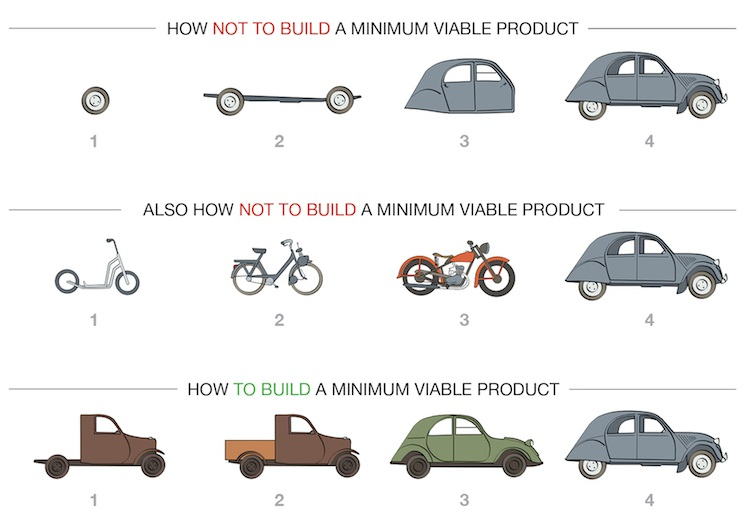
\includegraphics[width=0.75\columnwidth]{MVP}
	\caption{Framework to build an MVP (Fonte: \href{https://goo.gl/s8LmEH}{https://goo.gl/s8LmEH})}
\end{figure}

\subsection{Controllo di versione}
Come strumento di versionamento del codice, l’azienda utilizza \gls{Git}\footcite{https://git-scm.com/} ed in particolare, per poter gestire tutto il codice derivante dai vari progetti, il personale utilizza la versione \textit{enterprise} di \gls{GitLab}\footcite{https://about.gitlab.com/}, disponibile gratuitamente sotto licenza \textit{open source}.\\
Alcuni dei vantaggi che hanno spinto l’azienda ad utilizzare Git sono:
\begin{itemize}
	\item \textbf{Ridondanza}: ogni sviluppatore possiede una copia dell’intera \textit{repository}. Il rischio di perdita dei sorgenti del progetto è quindi inversamente proporzionale al numero di sviluppatori che ne possiedono in locale l’ultima versione; in caso di perdita del progetto di uno sviluppatore quindi si andrà incontro solamente alla perdita delle ultime modifiche personali fatte;
	\item \textbf{Disponibilità}: anche in assenza di connessione alla \textit{repository} principale, è possibile continuare ad effettuare \textit{commit} ed a salvare le modifiche fatte nel tempo. Una volta ripristinata la connessione, la \textit{repository} locale può essere sincronizzata con quella remota rendendo le modifiche disponibili a tutti;
	\item \textit{\textbf{Branch e Merge}}: permette con molta facilità la creazione di \textit{branch}, consentendo di creare quindi delle ramificazioni in cui sviluppare funzionalità non stabili, evitando di intaccare il ramo principale dove di norma risiede una versione stabile e testata del prodotto. Nel momento in cui lo sviluppatore vuole apportare le modifiche anche al ramo principale, \gls{Git} permette di effettuare l’operazione di \textit{merge} del nuovo ramo testato con il ramo principale e considerare quindi le ultime modifiche come stabili;
	\item \textit{\textbf{Fork e Pull request}}: queste due operazioni permettono di clonare una \textit{repository} (tramite \textit{fork}) e, successivamente, proporre l’inclusione delle modifiche apportate all’interno del clone nella \textit{repository} originale.
\end{itemize}
\begin{figure}[!h] 
	\centering 
	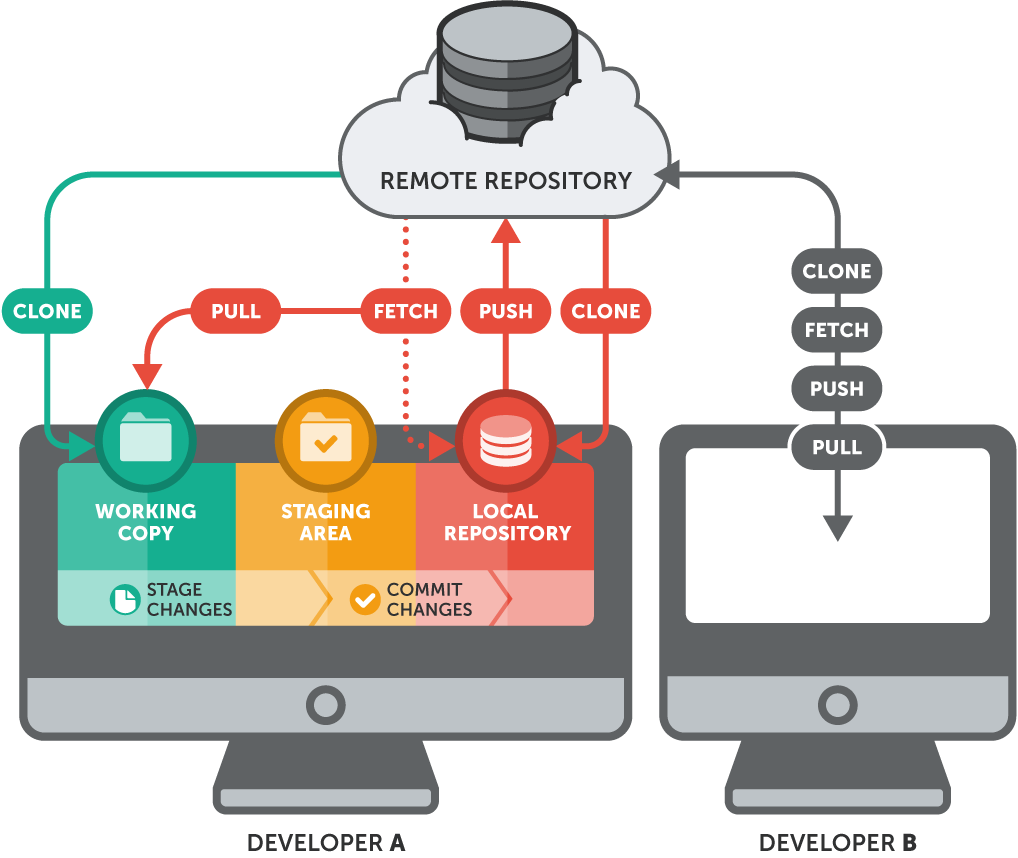
\includegraphics[width=0.7\columnwidth]{git} 
	\caption{Funzionamento ed operazioni in Git (Fonte: \href{https://goo.gl/m1PVZy}{https://goo.gl/m1PVZy})}
\end{figure}


\subsection{Ambiente di sviluppo}
Gli strumenti utilizzati per lo sviluppo, divisi in categorie, sono i seguenti:
\begin{itemize}
	\item \textbf{IntelliJ IDEA}\footcite{https://www.jetbrains.com/idea/}: è l'\gls{IDE} utilizzato in prevalenza dagli sviluppatori in quanto supporta vari linguaggi di programmazione e vari tool utili;
	\item \textbf{Visual Studio Code}\footcite{https://code.visualstudio.com/}: come il precedente, supporta vari linguaggi di programmazione e molteplici estensioni volte a migliorare lo sviluppo. A differenza del precedente, però, non supporta nativamente Java ed è quindi meno utilizzato;
	\item \textbf{\gls{Bash}}: per effettuare l'analisi dei dati preliminari, il team \textit{big data} utilizza la \textit{shell} di Linux per eseguire i tool interessati (ad esempio Hive, Impala, Spark o per visualizzare il \textit{filesystem} \gls{HDFS}).
\end{itemize}

%**************************************************************
\section{Propensione dell'azienda per l'innovazione}
L’azienda è alla continua ricerca di nuove tecnologie e prodotti innovativi che possano soddisfare sempre più le esigenze del cliente. Nel primo caso l’azienda cerca di cogliere il meglio delle nuove tecnologie per poterne trarre il maggior beneficio possibile attraverso progetti sperimentali e, per la prima volta quest’anno, stage universitari. Essendo l’innovazione un importante fattore di crescita, IT Euro Consulting coltiva questo aspetto cercando personale che abbia attitudine al cambiamento e contemporaneamente esprima le proprie soluzioni ai problemi incontrati dando libero sfogo alla propria creatività. Nel secondo caso, invece, l’azienda si prefigge l’obiettivo di creare nuovi prodotti al passo con le esigenze di potenziali clienti, utilizzando le ultime tecnologie disponibili.\\
Un'ulteriore prova della propensione all'innovazione dell'azienda è la presenza di un team specifico ed in continua espansione per il segmento \textit{big data}, cosa usuale all'estero ma ben più rara in Italia in aziende di medie dimensioni, nelle quali l'importanza dei dati e della potenzialità che essi possiedono non è ancora entrata pienamente nell'ideale di business delle aziende.
\begin{figure}[!h] 
	\centering 
	
\includegraphics[width=0.6\columnwidth]{Big_Data} 
	\caption{Attività dell'azienda in ambito big data (Fonte: \href{https://goo.gl/tyLXjo}{https://goo.gl/tyLXjo})}
\end{figure}             % Dove
%% !TEX encoding = UTF-8
% !TEX TS-program = pdflatex
% !TEX root = ../tesi.tex

%**************************************************************
\chapter{Lo stage nella strategia aziendale}
\label{cap:lo stage nella strategia aziendale}
%**************************************************************

\section{Aspettative personali}
La mia esperienza lavorativa si è sempre limitata a piccoli lavori occasionali, un periodo in cui ho svolto un progetto esterno per un'azienda ed in seguito uno stage nella stessa azienda, entrambi durante la scuola secondaria di secondo grado.\\
Già da queste piccole esperienze, avevo capito quanto la pratica sul campo fosse una valida opportunità per applicare attivamente quanto studiato durante la carriera da studente e, inoltre, apprendere nuove nozioni. 
Dall'attività di stage, quindi, le mie speranze erano quelle di poter apprendere nuove nozioni e consolidare quelle già in mio possesso tramite un approccio che fosse più pratico di quello che normalmente viene utilizzato all'interno dell'ambiente universitario. \\
I miei obiettivi iniziali per un progetto di stage erano quindi i seguenti:
\begin{itemize}
	\item Entrare in contatto con nuove tecnologie;
	\item Vedere e capire il funzionamento di una realtà aziendale in ambito tecnologico ed ICT;
	\item Poter lavorare con il supporto di personale qualificato;
	\item Vedere in pratica come le nozioni apprese in aula o da studio personale vengono realmente applicate nel mondo lavorativo.
\end{itemize}
Per far sì che le mie opzioni di scelta fossero quanto più numerose possibili, ho deciso di partecipare all'iniziativa denominata Stage-IT\footcite{http://informatica.math.unipd.it/laurea/stageit.html} organizzata dall'Università di Padova. Prima di andare all'evento, ho stilato una lista di possibili aziende a cui presentarmi, facendo soprattutto attenzione ai progetti proposti. Durante l'evento ho quindi colto l'occasione per discutere dell'attività di stage con molteplici aziende. Molte di loro operavano in campi che a mio parere non risultavano essere particolarmente interessanti, ma qualche azienda ha colto la mia curiosità e mi ha permesso di avere con loro un colloquio di presentazione reciproca. Alcune di queste erano più interessate a stage per inserimento lavorativo e di durata di circa 6 mesi, che ad uno finalizzato per la tesi, e quindi ho dovuto scartarle a priori nonostante il mio interesse. \\
Fortunatamente, l'azienda IT Euro Consulting proponeva uno stage adeguato per lo sviluppo della tesi e gli argomenti coinvolti erano pienamente di mio interesse: durante il colloquio conoscitivo comunque, l'azienda non mi ha subito presentato un progetto di stage, ma piuttosto mi ha esposto la struttura aziendale, la focalizzazione dello stage nell'ambito \textit{big data} e la propensione dell'azienda per l'innovazione e l'interesse a conoscere nuovi punti di vista come quello di uno studente universitario. Tutto ciò mi ha attratto fin da subito e quindi, dopo un paio di incontri successivi avvenuti in azienda, l'azienda ha proceduto alla presentazione del progetto di stage vero e proprio.

Considerando i miei obiettivi e la lista di aziende con le quali ho avuto un contatto a Stage-IT, ho deciso di svolgere il progetto di IT Euro Consulting, in quanto di maggiore interesse rispetto ai progetti offerti da altre aziende.

%**************************************************************
\section{Aspettative aziendali}
Quest'anno IT Euro Consulting ha deciso, per la prima volta, di attivare un progetto di stage universitario che non avesse come fine ultimo l'assunzione del tirocinante. I motivi di questa scelta sono molteplici e condivisibili. \\
In primo luogo è necessario distinguere i percorsi che l'azienda ha deciso di far intraprendere ai diversi tirocinanti in base allo scopo dello stage. \\ 
Per gli studenti, appena laureati o laureandi, il cui fine è l'assunzione al termine del tirocinio, l'azienda ha previsto un periodo di lavoro di circa 6 mesi, durante il quale, dopo il primo periodo formativo, lo stagista viene inserito in progetti già avviati e quindi affiancati dal team a cui è assegnato il lavoro. Negli ultimi 3 anni, infatti, l'azienda ha ampliato i reparti sviluppo e \textit{big data} ed ha assunto molteplici persone in seguito ad uno stage o tirocinio. Oggigiorno infatti la maggior parte del personale appartenente ai reparti sviluppo e \textit{big data} ha un titolo di laurea in Informatica o Ingegneria. \\
Nell'altro caso, ovvero lo stage curricolare, come di mio interesse, la durata è di circa 300-350 ore e si distingue in una fase di apprendimento ed in una fase di progetto, sempre affiancati da uno o più tutor interni. Durante il progetto, il tirocinante ha maggiore libertà sulla scelta delle tecnologie che utilizzerà e su decisioni progettuali. Queste poi vengono discusse con il tutor in modo da correggere eventuali scelte errate frutto dell'inesperienza del tirocinante. \\
I vantaggi di questi due percorsi sono in parte comuni: in primo luogo si ha l'inserimento in organico di nuove risorse provenienti dal mondo universitario. Assumere anche solo provvisoriamente una figura per uno stage proveniente dal mondo universitario giova all'azienda in quanto il personale ha la possibilità di confrontarsi ed aggiornarsi con costui sui nuovi insegnamenti e corsi universitari. Questa vicinanza è però anche utile per lo studente, in quando ha la possibilità di vedere concretamente come quanto appreso in aula sia implementato effettivamente nel mondo reale e di capire come funzioni realmente un'azienda, se non ha già avuto esperienze simili durante la sua carriera.
Il secondo motivo è la possibilità per l'azienda di comprendere il livello di preparazione medio degli studenti universitari ed essere attivi nello scrutare quelli più meritevoli che possono portare ad un vantaggio competitivo considerevole.
Per quanto riguarda il mio percorso di stage, quello curricolare, si possono riconoscere altri due vantaggi ed entrambi derivano dalla maggior libertà che si concede allo studente per risolvere problemi che solitamente in azienda si risolverebbero tramite soluzioni già consolidate. La possibilità di sfruttare nuove tecnologie senza la necessità di perdita di tempo del personale aziendale, permette di rimanere aggiornati sul continuo rilascio di librerie e \textit{framework} che potrebbero portare benefici ai vari team in termini di efficienza, sia sul tempo di sviluppo del software, sia per quanto riguarda le performance del prodotto stesso.
La maggiore libertà sulla progettazione e lo sviluppo concessa allo stagista consente anche di valutare vantaggi e svantaggi di soluzioni architetturali che il personale aveva scartato prematuramente o che non aveva considerato a priori.\\

Alla fine dello stage, l'azienda si aspettava di avere una \gls{web app} che esponesse i dati precedentemente recuperati dal \gls{cluster}, esaminati ed elaborati in modo da facilitare il successivo sviluppo del modello per stimare il target desiderato.

Tutto ciò mi ha portato prima dell'inizio dell'attività di stage, a concordare insieme al tutor aziendale i requisiti del progetto, che durante lo stage sono rimasti fedeli al Piano di Lavoro, senza dover effettuare cambiamenti imprevisti.
Per poter gestire al meglio lo stage ed avere una buona elasticità sugli obiettivi da raggiungere, il tutor li ha suddivisi in tre categorie: obiettivi obbligatori, obiettivi desiderabili e obiettivi facoltativi.

\begin{table}[!h] %
	\caption{Obiettivi dello stage} \label{obiettivi_stage}
	\label{tab:obiettivi-stage}
	\begin{tabular}{|l|}
		\hline
		\\[-2mm]
		\textbf{Obiettivi obbligatori}\\
		\hline
		\\[-2mm]
		Caricare, estrarre e compiere semplici operazioni su file presenti nel \gls{cluster}	\\
		\hline
		\\[-2mm]
		Svolgere semplici operazioni con Hive/Impala su tabelle già esistenti, con creazione \\ di nuove tabelle contenenti statistiche riassuntive e porzioni di dati	\\
		\hline
		\\[-2mm]
		Svolgimento di una semplice analisi dati con Spark, dall'ingestion all'esame del \\ \textit{dataset}, salvando i risultati in formato tabellare CSV	\\
		\hline
		\\[-2mm]
		Sviluppo di un \gls{Web Service} RESTful in grado di presentare in formato JSON i \\ risultati CSV \\
		\hline
		\hline
		\\[-2mm]
		\textbf{Obiettivi desiderabili}\\
		\hline
		\\[-2mm]
		Creazione di nuove tabelle tramite l'utilizzo di \textit{query} SQL innestate e con \\ operazioni complesse \\
		\hline
		\\[-2mm]
		Sviluppo di una semplice applicazione capace di interfacciarsi con i dati prodotti \\ da Spark e riassumere graficamente i risultati \\
		\hline
		\\[-2mm]
		Sviluppo di un'applicazione Java EE \textit{3-tier}, composta da un'interfaccia grafica \\ HTML5/Angular in grado di visualizzare i dati dei risultati in modalità grafica e \\ un Web Service RESTful per la presentazione dei dati in formato JSON recuperati \\ con Hive/Impala \\
		\hline
	\end{tabular}
\end{table}%
\clearpage
\begin{figure}[!h] 
	\centering 
	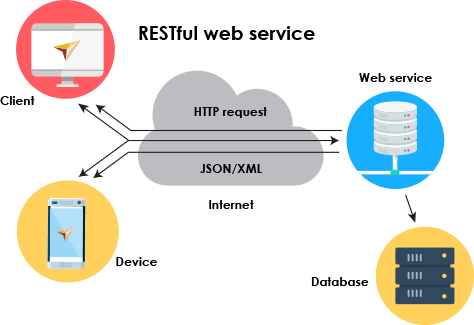
\includegraphics[width=0.75\columnwidth]{web-service}
	\caption{RESTful Web Service (Fonte: \href{https://goo.gl/zvrBJz}{https://goo.gl/zvrBJz})}
\end{figure}

%**************************************************************

\section{Presentazione del progetto}
Il progetto di stage oggetto di questa relazione è stato di natura esplorativa. Lo scopo dello stage è diviso in due parti:
\begin{itemize}
	\item Analisi ed elaborazione del \textit{dataset} e dei dati di interesse;
	\item Realizzazione di una \gls{web app} per la presentazione dei risultati ottenuti.
\end{itemize}
Il team \textit{big data} aveva già compiuto la prima attività circa 3 anni fa in occasione di un concorso a cui l'azienda aveva partecipato.
Grazie a questo stage, l'azienda ha dunque potuto esplorare l'utilizzo di metodi differenti per l'elaborazione e l'analisi dei dati rispetto a quelli utilizzati in precedenza. 
Inoltre, il personale potrà riutilizzare la \gls{web app} sviluppata in futuro come semplice interfaccia per dati e risultati finali di successivi progetti.
\subsection{Analisi ed elaborazione del dataset e dei dati di interesse}
Nella prima parte dello stage gli obiettivi erano molteplici. \\
In primo luogo l'azienda richiedeva allo stagista uno studio teorico sull'architettura del \gls{cluster}, sul funzionamento di Hadoop e la struttura di \gls{HDFS}, così da comprendere in pieno il funzionamento del sistema sottostante e di YARN, il tool che gestisce le risorse ed effettua lo \textit{scheduling} dei processi.
\clearpage
\begin{figure}[!h] 
	\centering 
	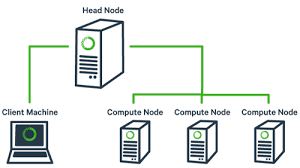
\includegraphics[width=0.65\columnwidth]{cluster}
	\caption{Rappresentazione di un cluster Hadoop (Fonte: \href{https://goo.gl/DgYJ4J}{https://goo.gl/DgYJ4J})}
\end{figure}

Il secondo obiettivo era lo studio dei tool principali che il team \textit{big data} utilizza per l'analisi ed il \textit{processing} dei dati, ovvero Hive, Impala, Spark. Oltre a questi tool di cui si è già dato un breve commento, l'azienda richiedeva lo studio di:
\begin{itemize}
	\item \textbf{Hue}\footcite{http://gethue.com/}: un'applicazione che offre un'interfaccia e semplifica alcune operazioni, come le \textit{query} su Hadoop, di cui è utile la conoscenza di base ma scarsamente utilizzato in quanto risulta relativamente complesso per utilizzi semplici;
	\item \textbf{Cloudera Manager}\footcite{https://www.cloudera.com/products/product-components/cloudera-manager.html}: una web app per la gestione dei servizi e dei tool di Hadoop. Permette di tenere sotto controllo il cluster, quindi le risorse disponibili e gli utenti collegati, e permette di gestire e visualizzare le attività dei tool attualmente in esecuzione e passati. È utilizzato principalmente dai \textit{system administrators} ma si rivela utile anche per il team \textit{big data} per un'analisi veloce del funzionamento \textit{real time} del sistema.
\end{itemize} 
\begin{figure}[!h] 
	\centering 
	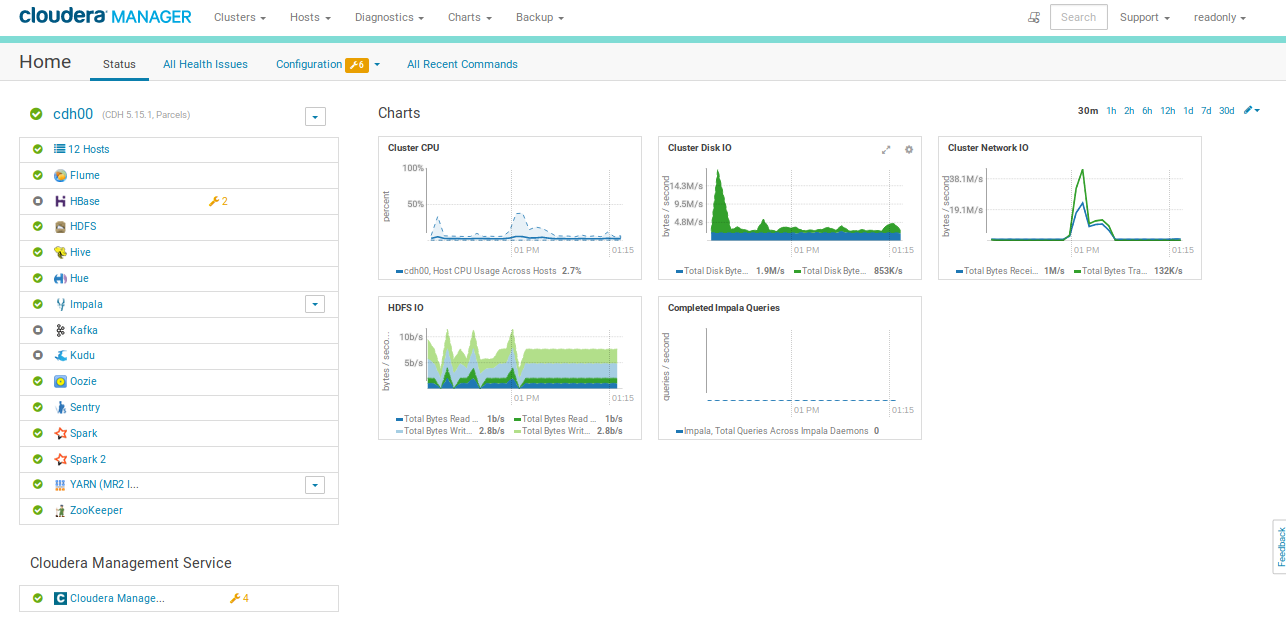
\includegraphics[width=1\columnwidth]{cloudera-manager}
	\caption{Interfaccia di Cloudera Manager}
\end{figure}
Al termine dello studio di questi tool, l'azienda richiedeva la comprensione e la successiva analisi del \textit{dataset} oggetto del progetto, che viene trattata in dettaglio nel capitolo successivo.
\subsection{Realizzazione di una web app per la presentazione dei risultati}
Dopo aver ottenuto tutti i dati di interesse, l'azienda richiedeva lo sviluppo di una \gls{web app} per la presentazione dei risultati in maniera più comprensibile ed appetibile rispetto a tabelle \gls{CSV} grezze. Grazie all'utilizzo di grafici, anche semplici, è infatti possibile notare alcune caratteristiche del \textit{dataset} che potrebbero rivelarsi utili ad una successiva analisi per la creazione del modello statistico.
%**************************************************************
\section{Vincoli}
\subsection{Vincoli metodologici}
Insieme con l'azienda, abbiamo deciso che avrei dovuto svolgere le attività di stage presso la sede della società. Questo è stato concordato con lo scopo di favorire il dialogo tra me ed il tutor aziendale e di avere la possibilità di confrontarmi direttamente con programmatori ed analisti più esperti in caso di problematiche durante lo svolgimento delle attività di progettazione, analisi e sviluppo software.
Oltre a ciò, l’azienda richiedeva che, al termine di ogni settimana lavorativa, venisse compilato un rapporto sulle attività che avevo svolto durante tale settimana. Inoltre, nel corso del primo periodo, prettamente di formazione, l'azienda richiedeva un breve resoconto di quanto compreso, cosicchè, in caso di dubbi, potessi confrontarmi con personale esperto prima di passare alla progettazione.
In seguito ad ogni rapporto, ed in particolare agli avanzamenti ed ai problemi incontrati descritti in esso, il tutor avrebbe deciso cosa avrei dovuto svolgere la settimana successiva, così da poter adattare al meglio il progetto al periodo di stage rimanente.\\
Al termine di tutte le attività, l'azienda richiedeva inoltre una breve presentazione di quanto svolto ad alcuni membri del management. Tale presentazione, esposta in forma verbale, mi sarebbe servita per illustrare ciò che avevo concluso tramite il progetto, elencando pro e contro della soluzione trovata.
\subsection{Vincoli temporali} \label{pdl}
Lo svolgimento dello stage prevedeva una durata di 320 ore complessive di lavoro. Queste ore sono state distribuite in modo uniforme in otto settimane lavorative da 40 ore ciascuna. Assieme al tutor aziendale, abbiamo concordato che l'orario di lavoro sarebbe stato dal Lunedì al Venerdì dalle 09:00 alle 18:00 con un'ora di pausa pranzo. Prima dell'inizio dello stage il tutor ha redatto nel Piano di Lavoro una scansione temporale delle attività su base settimanale.
In alcune occasioni, ho portato a termine il lavoro assegnato in anticipo, per cui abbiamo scelto di effettuare alcuni approfondimenti su argomenti che mi interessavano maggiormente, tramite lo studio autonomo ma con la possibilità di richiedere chiarimenti al personale più esperto che mi seguiva.
Il tutor ha quindi ripartito il lavoro su base settimanale nel seguente modo:
\begin{itemize}
	\item \textbf{Prima settimana}: 
		\subitem - consolidamento utilizzo sistema Unix;
		\subitem - comprensione mondo \textit{big data};
		\subitem - Apache Hadoop Architecture e \gls{HDFS}.
	\item \textbf{Seconda settimana}:
		\subitem - approfondimenti mondo \textit{big data};
		\subitem - apprendimento comandi \gls{HDFS};
		\subitem - comprensione tools Cloudera.
	\item \textbf{Terza settimana}:
		\subitem - approfondimento tools Cloudera;
		\subitem - studio ed esercitazione di Cloudera Impala ed Apache Hive.
	\item \textbf{Quarta settimana}:
		\subitem - studio ed esercitazione di Apache Spark;
		\subitem - comprensione di Cloudera Manager.
	\item \textbf{Quinta e sesta settimana}:
	 	\subitem - ripasso Java con attenzione all'ambiente Java EE;
	 	\subitem - studio del linguaggio scelto per il \textit{front-end}.
	\item \textbf{Settima e ottava settimana}:
		\subitem - applicazione delle principali tecnologie apprese al progetto.
\end{itemize}
Da questa suddivisione deriva il seguente \gls{Diagramma di Gantt}.
\begin{figure}[!h] 
	\centering 
	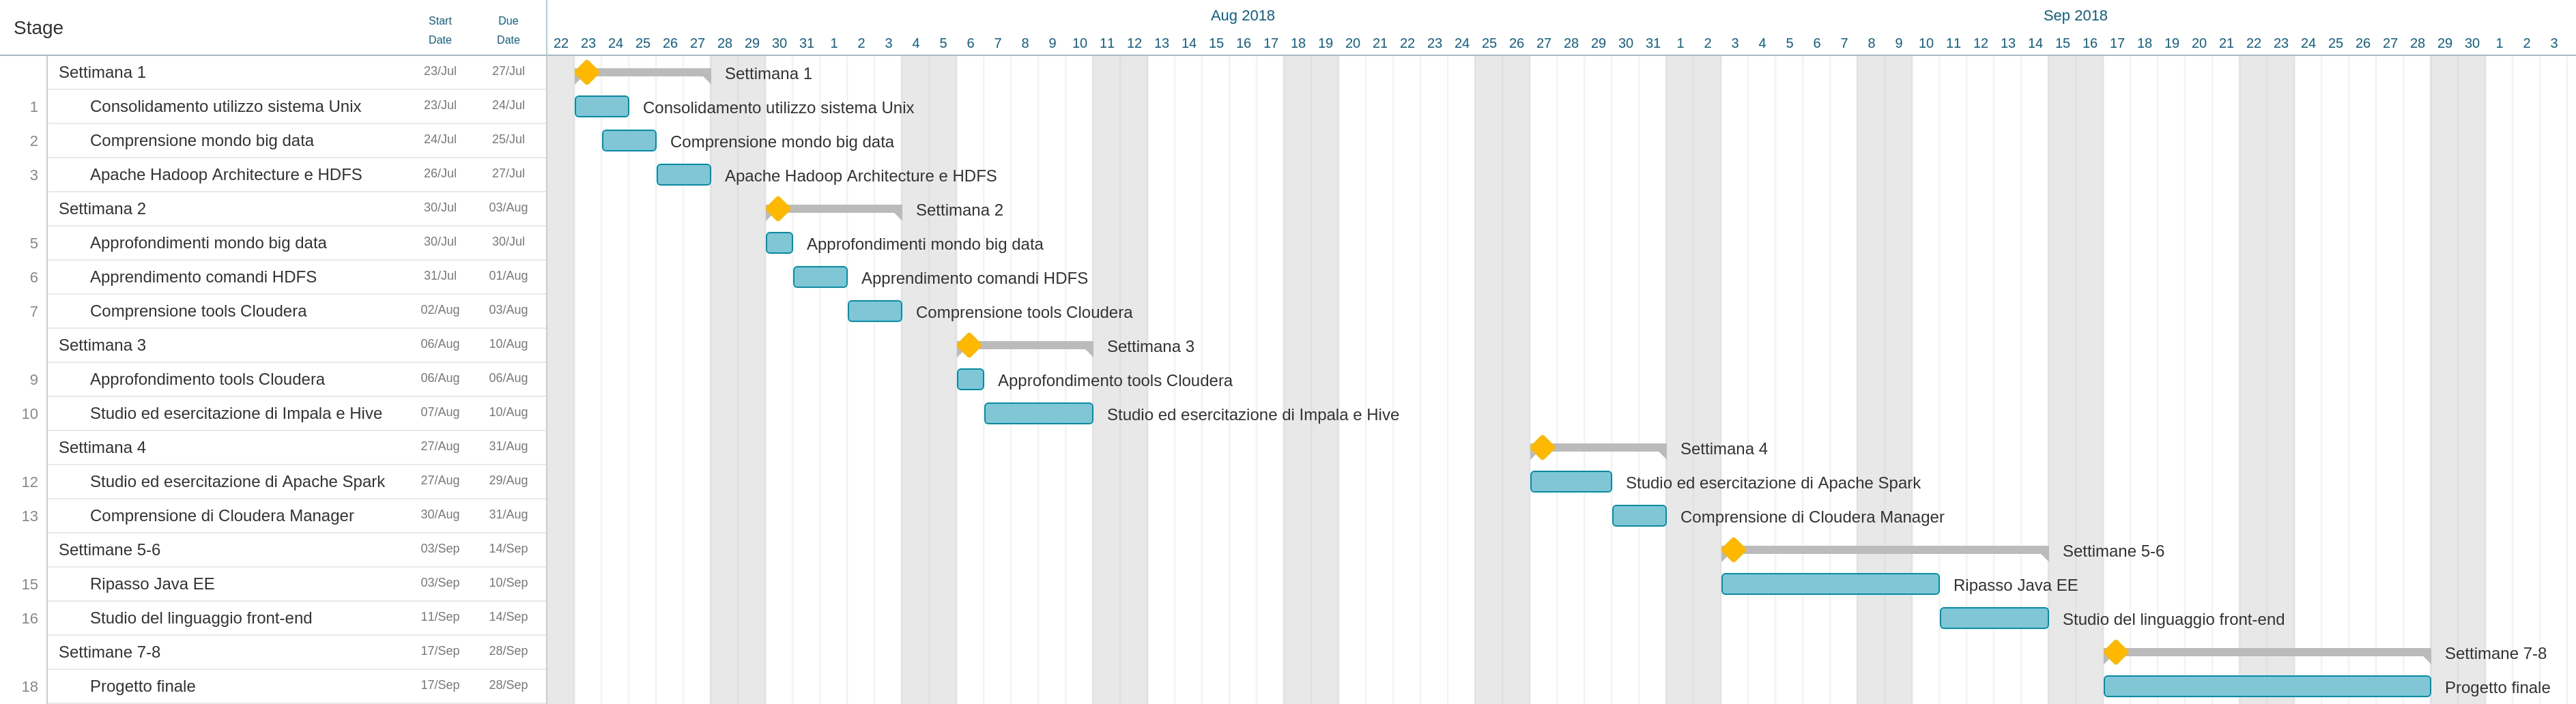
\includegraphics[width=1\columnwidth]{gantt}
	\caption{Diagramma di Gantt dello stage}
\end{figure}

\subsection{Vincoli tecnologici}
L'azienda, ad inizio stage, ha posto un unico vincolo per il progetto finale: utilizzare Java EE per la parte di \textit{back-end} del prodotto. Per la parte di \textit{front-end}, il tutor mi ha invece suggerito l'utilizzo di Angular, in quanto già assiduamente testato ed utilizzato per altri progetti, ma senza porre alcun tipo di vincolo, infatti la scelta finale dipendeva dalle mie preferenze ed esperienze passate. Inizialmente ho proposto come alternativa l'utilizzo delle librerie React\footcite{https://reactjs.org/} e Redux\footcite{https://redux.js.org/} in quanto già in parte conosciute ed utilizzate. Come decisione finale però ho scelto, come proposto dall'azienda, Angular, in  quanto mi interessava come tecnologia e, vista la natura esplorativa di nuove tecnologie e strumenti dello stage, l'ho considerata la scelta migliore per il mio accrescimento culturale. \\
Per quanto riguarda la parte di \textit{big data}, mi sono affidato completamente al mio tutor aziendale, in quanto non avevo alcuna esperienza in quel campo e quindi non avrei potuto scegliere cosa fosse la scelta migliore per me. Oltre a ciò, gli strumenti utilizzati assieme ad Hadoop sono ormai consolidati e non c'è una grande varietà, quindi la scelta proposta dal personale aziendale si è rivelata obbligatoria. \\
Oltre a ciò, ho avuto la possibilità di utilizzare \gls{Git} per il versionamento del codice, che ho ben apprezzato ed utilizzato.
%**************************************************************

% DA RIVEDERE COME MAIL PRIMA DI INVIARE CAP3
\section{Aspettative personali sul progetto di stage}
Successivamente al mio impegno con l'azienda ed alla stesura del Piano di Lavoro, assieme alla definizione degli obiettivi, la mia curiosità verso l'argomento di stage si è intensificata. \\
Le aspettative che maggiormente sentivo erano:
\begin{itemize}
	\item Mettersi in gioco in un'azienda con partner di un certo livello nel mio campo di studi;
	\item Instaurare con il personale discussioni su esperienze e punti di vista diversi sulle varie tecnologie;
	\item Entrare in contatto con tecnologie nuove e sempre più di largo utilizzo;
	\item Conoscere il funzionamento di uno strumento come Hadoop e tutti i tool inerenti;
	\item Apprendere come effettuare un'analisi su un insieme di dati distribuiti in un \gls{cluster};
	\item Imparare come progettare e quali sono le \textit{best practies} per realizzare una \gls{web app} utilizzando Java EE.
\end{itemize}             % Perchè
%% !TEX encoding = UTF-8
% !TEX TS-program = pdflatex
% !TEX root = ../tesi.tex

% (3) che risponde alle domande “cosa” e “come”, nel quale racconterai gli elementi essenziali del tuo stage,
% vedendolo come un mini‐progetto a se stante. In questo capitolo illustrerai: (a) il metodo di lavoro con il quale hai
% affrontato lo stage; (b) i problemi progettuali, tecnologici e applicativi che hai affrontati; (c) i risultati che hai
% raggiunto, sia sul piano qualitativo che su quello quantitativo. Il punto (a) comprende la pianificazione, le interazioni
% con il tutor aziendale, le revisioni di progresso, l’uso di diagrammi, di tecniche di analisi e tracciamento dei requisiti,
% l’uso di strumenti di verifica, ecc. Il punto (b), che tratterai nella sequenza di attività che hai svolto (analisi,
% progettazione, programmazione, verifica e validazione), metterà in luce gli aspetti principali, secondo una visione ad
% alto livello. Entrerai in dettaglio solo per aspetti che consideri particolarmente meritevoli di attenzione dal punto di
% vista delle conoscenze acquisite o necessarie. Il punto (c) tratta di copertura di requisiti, di copertura di testing, e di
% quantità di prodotti (linee di codice, numero di documenti, ecc.).


%**************************************************************
\chapter{Resoconto dello stage}
\label{cap:resoconto-stage}
%**************************************************************

\section{Descrizione del progetto}
Parte del progetto che l'azienda mi ha proposto era già stato sviluppato dal team \textit{big data} qualche anno fa.
Il \textit{dataset} da elaborare ed analizzare è infatti parte di un concorso a cui l'azienda aveva partecipato: questa competizione è stata indetta da BNP Paribas Cardif, il polo assicurativo del Gruppo BNP Paribas, e pubblicata su Keggle\footcite{https://www.kaggle.com/}, nota piattaforma in cui è possibile esporre i propri progetti, visualizzare quelli altrui e proporre sfide in ambito \textit{data science} e \textit{machine learning}.

\subsection{Il problema}
In particolare, il problema proposto, "BNP Paribas Cardif Claims Management"\footcite{https://www.kaggle.com/c/bnp-paribas-cardif-claims-management}, consiste nella possibilità di classificare le pratiche assicurative in modo che queste possano essere risolte nel minor tempo possibile. A tal proposito, si chiede di prevedere la categoria di un sinistro sulla base delle caratteristiche disponibili nelle prime fasi del processo assicurativo; le due categorie di richieste di indennizzo, su cui basare la classificazione, corrispondono quindi a:
\begin{itemize}
	\item Quelle per le quali l'approvazione poteva essere accelerata, con conseguente maggiore rapidità nel rimborso e minori pratiche da gestire;
	\item Quelle per le quali erano richieste informazioni supplementari prima dell'approvazione e del rimborso.
\end{itemize}
\clearpage
\begin{figure}[!h] 
	\centering 
	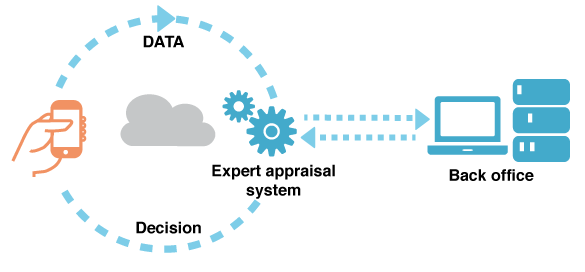
\includegraphics[width=0.7\columnwidth]{kaggle-project}
	\caption{Illustrazione del problema proposto (Fonte: \href{https://goo.gl/AW22at}{https://goo.gl/AW22at})}
\end{figure}
Nella sezione \hyperref[dataset]{Analisi del dataset di interesse} verrà trattata la struttura del \textit{dataset} più nel dettaglio.

%**************************************************************

\section{Studio di Hadoop e dei suoi tools}
Prima di cominciare a lavorare sul \textit{dataset} del progetto, era necessario studiare la teoria, in quanto la prima parte dello stage considerava argomenti a me quasi totalmente sconosciuti.
Autonomamente, ma sempre supervisionato dal tutor aziendale, disponibile a risolvere ogni mio dubbio, ho studiato il materiale necessario per poter eseguire poi al meglio la parte pratica. Oltre a ciò, nel corso della giornata lavorativa, il tutor mi sottoponeva delle esercitazioni da svolgere per consolidare i concetti appresi e risolvere tempestivamente miei eventuali dubbi prima di procedere con gli argomenti successivi.
Essendo \gls{HDFS} e molti dei tool Hadoop eseguibili principalmente tramite \gls{Bash}, come prima cosa mi è stato assegnato lo studio autonomo di alcuni capitoli, selezionati dal tutor, del libro "Learning the bash Shell"\footcite{http://shop.oreilly.com/product/9780596009656.do} per ottenere le basi che mi permettessero di utilizzare i comandi che mi sarebbero serviti in seguito per l'utilizzo dei tool Hadoop.\\
Dopo aver assorbito i concetti, già in parte di mia conoscenza, il tutor mi ha esposto la struttura del \gls{cluster} Hadoop in cui risiedevano i dati e venivano eseguiti i \textit{task}. 
\subsection{Apache Hadoop}
Ogni giorno si generano petabytes di dati che, se processati ed analizzati a dovere possono offrire informazioni con un alto valore strategico per un'azienda. Hadoop nasce dall'esigenza di dover gestire e processare questi dati in modo veloce, tramite una soluzione che sia il più possibile economica e scalabile orizzontalmente: aggiungendo nuovi nodi al cluster, la capacità e le performance di questo infatti aumentano proporzionalmente. Per aumentare ulteriormente le prestazioni e la scalabilità del sistema, Hadoop cerca di elaborare i dati sullo stesso nodo in cui questi risiedono: questo permette di ridurre al minimo la \textit{cross-communication} fra i nodi e la necessità di copiare grandi quantità di dati fra questi, eliminando il rischio di \textit{bottleneck} dovuto dalla velocità di trasmissione dei dati. Per gestire il sistema, Hadoop si basa su:
\begin{itemize}
	\item \gls{HDFS}: per la gestione dei dati persistenti;
	\item YARN: per lo \textit{scheduling} dei processi (\textit{jobs}) e la gestione delle risorse.
\end{itemize}
\begin{figure}[!h]
	\centering 
	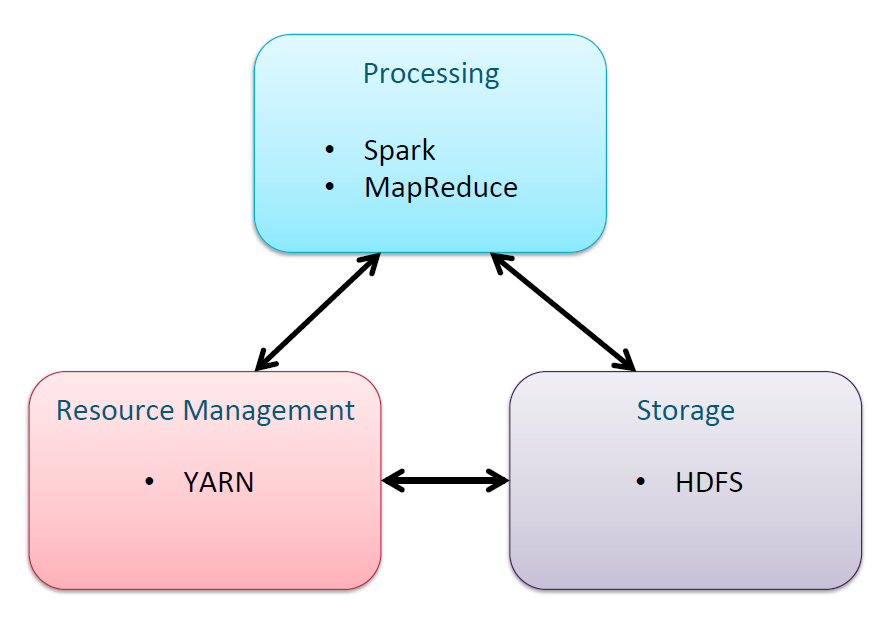
\includegraphics[width=0.7\columnwidth]{hadoop_tools}
	\caption{Attori principali del sistema Hadoop (Fonte: Cloudera - Developer Training for Spark and Hadoop)}
\end{figure}
\subsubsection{HDFS}
Hadoop Distributed File System (HDFS) è un \textit{file system} scritto in Java, basato su Google File System\footcite{https://ai.google/research/pubs/pub51}. \\
Offre performance migliori con un modesto numero di file di grandi dimensioni piuttosto che miliardi di dati frammentati, per questo motivo, anche le operazioni di \textit{read}, sono ottimizzate per la lettura in \textit{streaming} piuttosto che quelle casuali. Inoltre, i file sono tutti \textit{write-once} e quindi non modificabili una volta memorizzati.
In scrittura, infatti, i dati sono suddivisi in blocchi di dimensione fissata e distribuiti tra i nodi una volta caricati in modo ridondante per prevenire la perdita di informazioni nel caso un nodo non fosse più disponibile in seguito.
\begin{figure}[!h]
	\centering
	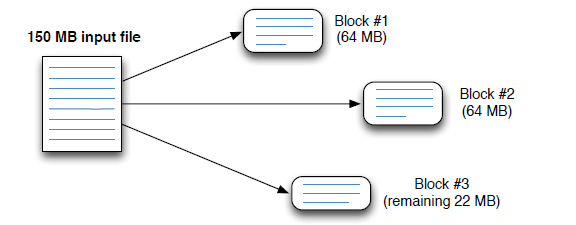
\includegraphics[width=0.8\columnwidth]{data_split}
	\caption{Divisione di un file in blocchi su HDFS (Fonte: Cloudera - Administrator Training for Apache Hadoop)}
\end{figure}
\clearpage
\begin{figure}[!h]
	\centering
	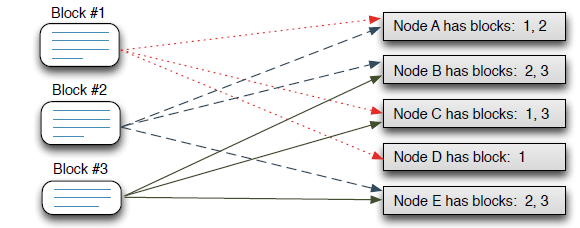
\includegraphics[width=0.8\columnwidth]{data_save}
	\caption{Caricamento dei blocchi nei nodi (Fonte: Cloudera - Administrator Training for Apache Hadoop)}
\end{figure}
Hadoop ha un'architettura di tipo \textit{master-slave}, ovvero in cui il processo \textit{master} ha il controllo su quello \textit{slave}. I nodi, quindi, possono essere di tre tipi:
\begin{itemize}
	\item \textbf{NameNode}: costituisce il \textit{master \gls{daemon}}, quindi gestisce tutti i \textit{metadata}, le informazioni riguardo l'\textit{ownership} e i permessi ad una risorsa, i nomi dei blocchi e la loro locazione;
	\item \textbf{DataNode}: costituisce gli \textit{slave \gls{daemon}}, quindi i nodi che contengono i blocchi di dati;
	\item \textbf{Secondary NameNode}: ha il ruolo di \textit{backup} del NameNode e quindi costituisce il \textit{master \gls{daemon}} di riserva. 
\end{itemize}
\begin{figure}[!h]
	\centering
	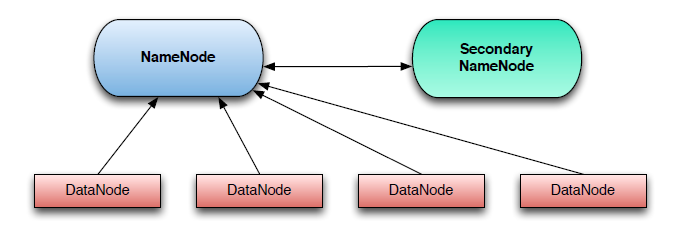
\includegraphics[width=0.8\columnwidth]{hadoop-nodes}
	\caption{Rappresentazione dei nodi in Hadoop (Fonte: Cloudera - Administrator Training for Apache Hadoop)}
\end{figure}
%La struttura del file system è basata su quella del sistema operativo sottostante e può essere ext3, ext4 o xfs 
\subsubsection{YARN}


\subsection{Apache Hive, Apache Spark e Cloudera Impala}

%**************************************************************
\section{Analisi del dataset di interesse} \label{dataset}

%**************************************************************

\section{Progettazione e sviluppo della web app}
             % Cosa/come
%% !TEX encoding = UTF-8
% !TEX TS-program = pdflatex
% !TEX root = ../tesi.tex

%**************************************************************
\chapter{Valutazione retrospettiva}
\label{cap:valutazione-retrospettiva}
%**************************************************************

\section{Soddisfacimento degli obiettivi}
Prima dell'inizio dell'attività di stage, io e il mio tutor abbiamo redatto il Piano di Lavoro. All'interno di esso, oltre ad una sintesi dell'organizzazione del tirocinio e ad una serie di ulteriori informazioni, abbiamo fissato anche gli obiettivi obbligatori e desiderabili che avrei dovuto raggiungere nell'arco delle 320 ore di stage, visibili in \hyperref[obiettivi_stage]{questa} tabella.\\
Gli obiettivi desiderabili che abbiamo fissato erano tutti degli incrementi rispetto a quelli obbligatori. In questo modo mi sarei potuto concentrare su quelli più importanti per primi e solo in seguito, una volta finiti, approfondire gli altri.\\ 
Sono riuscito a raggiungere tutti gli obiettivi obbligatori e parzialmente quelli desiderabili. Di quest'ultimi, infatti ho solo in parte soddisfatto il seguente:
\begin{itemize}
	\item Sviluppo di un'applicazione Java EE \textit{3-tier}, composta da un'interfaccia grafica HTML5/Angular in grado di visualizzare i dati dei risultati in modalità grafica e un Web Service RESTful per la presentazione dei dati in formato JSON recuperati con Hive/Impala.
\end{itemize}
Questo perchè, come precedentemente già descritto, zsdkòoiljndegrfaslkijmnsvfbdòlknsfdgòlknfxdbv


\section{Conoscenze acquisite}


\section{Valutazione personale}             % Valutazione retrospettiva
\appendix                               
% % !TEX encoding = UTF-8
% !TEX TS-program = pdflatex
% !TEX root = ../tesi.tex

%**************************************************************
\chapter{Appendice A}
%**************************************************************

\epigraph{Citazione}{Autore della citazione}



             % Appendice A

%**************************************************************
% Materiale finale
%**************************************************************
\backmatter
\printglossaries
%% !TEX encoding = UTF-8
% !TEX TS-program = pdflatex
% !TEX root = ../tesi.tex

%**************************************************************
% Bibliografia
%**************************************************************

\cleardoublepage
\chapter{Bibliografia}

\nocite{*}
% Stampa i riferimenti bibliografici
\printbibliography[heading=subbibliography,title={Riferimenti bibliografici},type=book]

% Stampa i siti web consultati
\printbibliography[heading=subbibliography,title={Siti web consultati},type=online]


\end{document}
